\documentclass[11pt,a4paper]{article}
\usepackage[utf8]{inputenc}
\usepackage[T1]{fontenc}
\usepackage[french]{babel}
\usepackage{lmodern}
\usepackage[margin=2.3cm]{geometry}
\usepackage{amsmath,amssymb}
\usepackage{booktabs}
\usepackage{graphicx}
\usepackage{listings}
\usepackage{xcolor}
\usepackage[hidelinks]{hyperref}
\usepackage{caption}
\usepackage{subcaption}
\usepackage{float}

\lstset{basicstyle=\ttfamily\small, columns=fullflexible, keepspaces=true,
        frame=single, breaklines=true, xleftmargin=3pt, xrightmargin=3pt,
        rulecolor=\color{gray!50}, backgroundcolor=\color{gray!5},
        language=C, keywordstyle=\color{blue!60!black}, commentstyle=\color{green!40!black}}
\newcommand{\code}[1]{\texttt{#1}}
\newcommand{\cs}{\mathit{cs}}

\title{Optimisation des échantillonneurs exacts en précision arbitraire\\[2pt]
\large Versions \code{\_opt} des cinq algorithmes du pipeline}
\author{Dépôt \code{FLDR-experiments}}
\date{19 octobre 2026}

\begin{document}
\sloppy
\maketitle

\begin{abstract}
Nous proposons une version optimisée de chacun des cinq échantillonneurs comparés
dans la figure~4 de l'article (Integer-Alias, FLDR, ALDR, Rust-Alias et
Fraction-Alias, tous en précision arbitraire), ainsi qu'un nouveau producteur de
bits aléatoires. Chaque version garde la philosophie de son algorithme (même table
ou même arbre, mêmes opérations exactes, fractions conservées pour Fraction-Alias,
uniforme sur $[0, W)$ pour Rust-Alias) et consomme exactement le même nombre de bits
aléatoires. Dans les conditions du pipeline, le tirage est de \textbf{20 à 61 fois
plus rapide} selon l'algorithme ; la mémoire baisse de 28 à 78\,\% pour quatre
algorithmes sur cinq. Ce travail a aussi mis au jour \textbf{un bug dans le FLDR GMP
d'origine}, qui échantillonnait une distribution biaisée ; il a été corrigé et
remesuré. Les autres algorithmes d'origine n'ont pas été modifiés. Enfin, une variante
\code{alias.integers\_v2} remplace l'uniforme et le Bernoulli de Lumbroso par un seul
mot de 64 bits par tirage : environ 2 fois plus rapide qu'\code{alias.integers\_opt},
pour 64 bits par tirage au lieu de 17,6 (section~\ref{sec:v2}).
\end{abstract}

\section{Résumé des résultats}

\begin{table}[H]
\centering
\small
\begin{tabular}{lrrrrr}
\toprule
Algorithme & \multicolumn{2}{c}{Temps médian / tirage} & Gain & Mémoire & Bits / tirage \\
\cmidrule(lr){2-3}
 & original & optimisé & (min--max) & (médiane) & (identiques) \\
\midrule
Integer-Alias  & 594 ns  & 13,3 ns & $\times 45$ (32--51) & $-28\,\%$ & 17,59 \\
FLDR$^*$       & 664 ns  & 33,6 ns & $\times 20$ (15--29) & $-78\,\%$ & 10,66 \\
ALDR           & 599 ns  & 16,6 ns & $\times 37$ (21--50) & $-78\,\%$ & 8,29 \\
Rust-Alias     & 1918 ns & 62,6 ns & $\times 30$ (26--36) & $+9\,\%$  & 185,20 \\
Fraction-Alias & 747 ns  & 12,4 ns & $\times 61$ (38--69) & $-30\,\%$ & 17,59 \\
\bottomrule
\end{tabular}
\caption{Résultats sur les 201 distributions du protocole de la figure~4
($n = 20\,484$, $w \approx 4{,}7\cdot 10^{50}$, $10^7$ tirages, 14 exécutions
parallèles). Les gains sont calculés distribution par distribution.
$^*$FLDR original après correction du bug (section~\ref{sec:fldr}).}
\label{tab:resume}
\end{table}

Ces gains viennent de deux sources, qu'on peut séparer sur Integer-Alias
(distribution \code{d.00100}, exécution seule, $10^7$ tirages) :
l'algorithme optimisé avec l'ancien producteur de bits passe de 3,83~s à 0,56~s
($\times 6{,}8$), puis le nouveau producteur le ramène à 0,10~s ($\times 5{,}4$),
soit $\times 37$ au total.

\section{Pourquoi le pipeline ralentissait les mesures}
\label{sec:pipeline}

Le pipeline lance 14 mesures en parallèle. Nous avons mesuré la même distribution en
faisant varier le nombre de mesures simultanées (temps \code{clock()} pour
$10^7$ tirages, avec l'ancien producteur de bits) :

\begin{table}[H]
\centering
\small
\begin{tabular}{rrr}
\toprule
Mesures en parallèle & Integer-Alias optimisé & Integer-Alias original \\
\midrule
1  & 0,56 s & 3,83 s \\
5  & 0,92 s & 5,44 s \\
10 & 1,65 s & 6,12 s \\
14 & 1,96 s & 8,10 s \\
\bottomrule
\end{tabular}
\end{table}

\noindent Trois causes s'additionnent.
\begin{enumerate}
\item \textbf{Surcharge du processeur.} Chaque mesure a deux threads : le tirage et le
  producteur de bits. Avec 14 mesures, cela fait 28 threads actifs pour 14 cœurs,
  dont 4 cœurs « efficacité » nettement plus lents que les 10 cœurs « performance »
  de l'Apple M4.
\item \textbf{L'ancien producteur ne s'arrête jamais.} Quand son buffer de 64 mots est
  plein, il boucle sur \code{sched\_yield()} et occupe un cœur en permanence. Or
  \code{clock()} additionne le temps CPU de tous les threads du processus : ce temps
  perdu est compté dans le temps de tirage, et il augmente quand la machine est chargée.
\item \textbf{Ressources partagées.} Le ralentissement apparaît dès 5 mesures, alors
  qu'il reste des cœurs performance libres : les mesures se disputent aussi le cache
  et la mémoire. Chaque mesure balaie par exemple 128~Mo (\code{flush\_cache}) au
  début et à la fin, pendant que les autres mesurent. En charge, la fréquence des
  cœurs baisse également.
\end{enumerate}
Le protocole reste identique pour tous les algorithmes, donc la comparaison reste
équitable ; mais les temps absolus sont gonflés, d'autant plus que l'algorithme est
rapide. Le nouveau producteur (section~\ref{sec:producteur}) supprime la deuxième
cause pour les versions optimisées. La part exacte de la troisième cause n'a pas été
isolée.

\section{Le nouveau producteur de bits aléatoires}
\label{sec:producteur}

L'ancien producteur (\code{flip.c}) appelle \code{arc4random\_buf} pour chaque mot de
32 bits. Chaque appel coûte environ 39~ns, alors qu'un appel sur un bloc de 4~Ko
coûte 0,8~ns par mot de 32 bits :

\begin{table}[H]
\centering
\small
\begin{tabular}{rr}
\toprule
Taille du bloc (mots de 64 bits) & Coût par mot de 32 bits \\
\midrule
1 & 14,3 ns \\
8 & 9,9 ns \\
64 & 1,8 ns \\
512 & 0,8 ns \\
\bottomrule
\end{tabular}
\end{table}

Le nouveau producteur (\code{c/flip\_opt.c} et \code{c/flip\_opt.h}) garde le même
principe, un thread qui remplit en continu un buffer de bits cryptographiques
(\code{arc4random}), avec les changements suivants :
\begin{itemize}
\item un buffer circulaire de 256~Ko en mots de 64 bits, rempli par blocs de 512 mots ;
\item \code{head} et \code{tail} sur des lignes de cache distinctes, publiés avec une
  sémantique \emph{acquire/release} ; le consommateur ne relit \code{tail} que
  lorsqu'il a épuisé les mots qu'il sait disponibles ;
\item quand le buffer est plein, le producteur dort 50~µs au lieu de boucler. Le buffer
  contient environ deux millions de bits, soit plusieurs millisecondes de tirages ;
\item le consommateur lit les bits directement dans le mot courant (fonctions
  \emph{inline}), avec \code{ctz} pour trouver la première pièce égale à 1.
\end{itemize}
Les bits sont lus du poids faible vers le poids fort, comme dans \code{flip.c}. Le
compteur \code{NUM\_RNG\_CALLS} est incrémenté de 2 par mot de 64 bits : la colonne
« bits » du pipeline garde donc la même unité.

\code{main.c} choisit le producteur d'après le nom de l'échantillonneur : les
échantillonneurs dont le nom se termine par \code{\_opt} utilisent le nouveau,
les autres gardent \code{flip.c}, qui n'a pas été modifié.

\section{Optimisations par algorithme}

Les cinq versions optimisées partagent deux briques, définies dans \code{flip\_opt.h}.

\paragraph{Uniforme sur $[0, n)$.} Même Fast Dice Roller de Lumbroso que
\code{uniform} et \code{uniform\_with\_gmp}, sur des entiers machine (l'indice d'une
cellule tient sur 32 bits), avec le nombre de bits du premier bloc précalculé.

\paragraph{Bernoulli($t/d$) à chiffres précalculés.} Le Bernoulli de Lumbroso tire des
pièces $c_1, c_2, \ldots$ et renvoie le chiffre binaire $d_k$ de $t/d$ à la première
pièce $c_k = 1$ ; si le développement se termine exactement au chiffre $k$, il renvoie
directement $c_k$. On a donc $\Pr(1) = \sum_k d_k 2^{-k} = t/d$. Au prétraitement, on
calcule une fois pour toutes
\[
D = \left\lfloor t\cdot 2^{31}/d \right\rfloor = (d_1\ldots d_{31})_2,
\qquad \rho = t\cdot 2^{31} \bmod d,
\]
et on stocke les 31 chiffres, plus un drapeau qui vaut 1 si $\rho = 0$. Au tirage, on
cherche la première pièce égale à 1 avec \code{ctz}, puis :
\begin{itemize}
\item si le développement est fini et se termine au chiffre $L$, on lit au plus $L$
  pièces. Si la première pièce à 1 est en position $k \le L$, on renvoie $d_k$ ; pour
  $k = L$ c'est bien $c_L = 1$. Si les $L$ pièces sont nulles, on renvoie $0 = c_L$ ;
\item sinon, si la première pièce à 1 est en position $k \le 31$, on renvoie $d_k$ ;
\item si les 31 premières pièces sont nulles (probabilité $2^{-31}$), on reprend la
  boucle GMP d'origine à partir de l'état $\rho$. Le résultat reste exact.
\end{itemize}
Les pièces sont lues dans le même ordre et en même nombre que dans l'original.

\subsection{Integer-Alias (\code{alias.integers\_opt})}
\begin{itemize}
\item Même table que l'Algorithme~1 de l'article, construite dans le même ordre
  (piles $L$ et $S$, LIFO, objet virtuel), et même rejet de l'objet virtuel.
\item Uniforme et Bernoulli($T[i]/\cs$) selon les deux briques ci-dessus : plus aucune
  opération GMP au tirage, sauf dans le repli de probabilité $2^{-31}$.
\item Cellules de 16 octets (chiffres, objet, alias, position du seuil). Les seuils
  exacts sont stockés en octets, uniquement pour les cellules avec alias, rangées en
  tête de table ; l'ordre des cellules est indifférent puisqu'elles sont tirées
  uniformément.
\end{itemize}

\subsection{FLDR (\code{rej.enc\_opt})}
\begin{itemize}
\item Même arbre DDG que \code{rej.enc\_gmp}, lu dans le même fichier (encodage
  \code{pack\_tree} construit en Python à partir des poids en précision arbitraire),
  parcouru comme dans le FLDR de Saad (\code{sample\_rejection\_encoding}).
\item L'encodage ne contient que des positions mémoire et des étiquettes : il est stocké
  en \code{int32} au lieu de \code{mpz\_t} (les valeurs sont vérifiées à la lecture).
\item Le parcours avance bit par bit dans le mot courant, sans appel de fonction par bit.
\end{itemize}

\subsection{ALDR (\code{aldr\_opt})}
\begin{itemize}
\item Même arbre aplati que \code{aldr\_gmp} (profondeur $K = 2k$, facteur
  $c = \lfloor 2^K/m \rfloor$). La construction d'origine recalcule le produit GMP
  $c\cdot a_i$ pour chacun des $K+1$ niveaux, soit environ $336 \times 20\,484$
  multiplications ; la version optimisée le calcule une fois par objet, dans le même
  ordre. Les arbres obtenus sont identiques (vérifié sur 3\,000 distributions).
\item Les largeurs de niveau et les feuilles sont stockées en \code{uint32}. Les
  compteurs du parcours tiennent en entiers machine, car un arbre DDG a au plus $n+1$
  nœuds internes par niveau.
\item Parcours bit par bit dans le mot courant.
\end{itemize}

\subsection{Rust-Alias (\code{alias.rust\_opt})}
\begin{itemize}
\item Même table que \code{alias.rust\_gmp} (construite par \code{weighted\_alias\_new\_gmp} :
  poids multipliés par $n$, cellules de capacité $W$).
\item Même tirage, fidèle à la crate Rust : une cellule uniforme, puis un entier
  \emph{uniforme sur $[0, W)$ en précision arbitraire} (environ 185 bits), comparé au
  seuil. Nous avons volontairement gardé cet uniforme complet, qui fait le coût en bits
  de cette méthode.
\item L'uniforme sur $[0, W)$ suit le même Fast Dice Roller, mais sur des entiers GMP
  préalloués (aucune allocation par tirage), avec les limbs aléatoires écrits
  directement. Les seuils sont stockés en limbs contigus de largeur fixe.
\item La mémoire augmente de 9\,\%. Les seuils sont stockés à largeur fixe (celle de
  $W$), alors que la mesure d'origine ne compte que les octets utiles de chaque entier ;
  s'y ajoutent les deux entiers de travail préalloués.
\end{itemize}

\subsection{Fraction-Alias (\code{alias.fractions\_opt})}
\begin{itemize}
\item Même table que \code{alias.fractions\_gmp} (construction de Vose sur des
  probabilités rationnelles exactes). \textbf{Les fractions sont conservées} : chaque
  cellule garde son numérateur et son dénominateur exacts, et le Bernoulli($a/b$)
  utilise les 31 premiers chiffres binaires de la fraction, avec repli exact sur la
  fraction elle-même.
\item Cellules de 16 octets ; numérateurs et dénominateurs en octets, uniquement pour
  les cellules avec alias.
\end{itemize}

\section{Le bug du FLDR GMP d'origine}
\label{sec:fldr}

L'encodage FLDR (\code{pack\_tree}, Saad et al.) range une feuille dans \emph{une} case
(\code{[-label]}) et un nœud interne dans deux cases (positions de ses enfants). Le
parcours correct, celui de \code{sample\_rejection\_encoding}, est :
\begin{lstlisting}
c = enc[c + b];          // position de l'enfant
if (enc[c] < 0) ...      // feuille : etiquette -enc[c]
\end{lstlisting}
La version GMP d'origine (\code{sample\_ky\_encoding\_gmp}) testait \code{enc[c + b] < 0}.
Arrivée sur une feuille, elle lisait donc un bit de plus : avec ce bit à 0 elle trouvait
bien la feuille, mais avec ce bit à 1 elle lisait la case suivante, qui appartient à un
autre nœud. Le parcours repartait alors d'un mauvais endroit.

\begin{table}[H]
\centering
\small
\begin{tabular}{llrrr}
\toprule
Distribution & Version & p-valeur $\chi^2$ & Pire objet (obs. / attendu) & Bits / tirage \\
\midrule
\code{d.00100} & GMP d'origine & 0 & 31\,732 / 52\,066 & 12,97 \\
\code{d.00100} & GMP corrigée  & 0,23 & conforme & 10,67 \\
\code{d.00180} & GMP d'origine & 0 & 804 / 1\,634 & 18,64 \\
\code{d.00180} & GMP corrigée  & 0,45 & conforme & 16,50 \\
\bottomrule
\end{tabular}
\caption{$2\cdot 10^6$ tirages par cas, comparés aux probabilités exactes $w_i/w$.}
\end{table}

\noindent Conséquences sur les résultats de l'article :
\begin{itemize}
\item la distribution échantillonnée par « FLDR (GMP) » n'était pas la bonne ;
\item sa consommation de bits était surestimée d'environ 2,2 bits par tirage
  (12,88 en moyenne au lieu de 10,66) ;
\item son temps était \emph{sous-estimé} : 492~ns en médiane dans la série biaisée,
  664~ns après correction.
\end{itemize}

La correction change trois lignes de \code{c/sample.c}.
Elle a été validée de deux façons : sur un flux de bits identique, la version corrigée
donne le même résultat et consomme le même nombre de bits que le FLDR de Saad
(250\,000 tirages sur 5 fichiers, 0 divergence) ; et elle passe le test du $\chi^2$.
\code{rej.enc\_gmp} a ensuite été remesuré dans les conditions du pipeline.

\section{Validation}

\subsection{Équivalence chemin par chemin}

Un test remplit l'ancienne file de bits (mots de 32 bits) et la nouvelle (mots de
64 bits) avec exactement la même suite de bits, exécute l'original puis la version
optimisée, et compare le résultat et le nombre de bits consommés.

\begin{table}[H]
\centering
\small
\begin{tabular}{lrr}
\toprule
Composant comparé à l'original & Cas testés & Divergences \\
\midrule
Bernoulli à chiffres précalculés vs \code{bernoulli\_with\_gmp} & 397\,847 & 0 \\
\quad dont repli GMP (31 chiffres / 3 chiffres) & 119\,020 / 254\,975 & 0 \\
Uniforme vs \code{uniform} & 126\,669 & 0 \\
ALDR : arbre et tirages vs \code{aldr\_gmp} (3\,000 arbres) & 60\,000 & 0 \\
FLDR optimisé vs FLDR de Saad (4 fichiers) & 80\,000 & 0 \\
FLDR GMP corrigé vs FLDR de Saad (5 fichiers) & 250\,000 & 0 \\
\bottomrule
\end{tabular}
\end{table}

\noindent Les seuils testés vont de 1 à 400 bits, dont un quart avec un développement
binaire fini ; les flux de bits sont uniformes, peu denses ou très creux, pour
provoquer de longues suites de zéros. La version « 3 chiffres » force le repli GMP.
Pour l'uniforme, la comparaison chemin par chemin n'a de sens que si le premier bloc
de bits ne franchit pas une frontière de mot de 32 bits : au-delà, l'ancienne et la
nouvelle file assemblent les mêmes bits dans un ordre différent, et les deux résultats
restent uniformes.

Pour Integer-Alias, Rust-Alias et Fraction-Alias, l'ordre des cellules ou celui des
limbs aléatoires diffère de l'original, et la comparaison chemin par chemin ne
s'applique pas directement. Leur exactitude repose sur les tests ci-dessus pour leurs
briques communes, et sur les tests statistiques qui suivent.

\subsection{Tests statistiques}

Les dix échantillonneurs (cinq originaux, cinq optimisés) ont été testés par un
$\chi^2$ contre les probabilités exactes, sur trois distributions réelles du protocole
(entropies basse, moyenne et haute), avec $2\cdot 10^6$ tirages chacun et le vrai
producteur de bits. Toutes les p-valeurs sont compatibles avec une distribution exacte
(de 0,06 à 0,98) ; aucun tirage hors support. La consommation de bits de chaque version
optimisée coïncide avec celle de son original.

Pour Integer-Alias, l'uniformité des p-valeurs a aussi été vérifiée sur 40 répétitions
(test de Kolmogorov--Smirnov : $p = 0{,}28$ pour la version optimisée, $0{,}88$ pour
l'original).

\section{Mesures expérimentales}

Protocole de la figure~4 : 201 distributions de \code{experiments/}\allowbreak
\code{distributions\_entropy}, $10^7$ tirages par distribution, 14 mesures en
parallèle, deux passes, MacBook Pro Apple M4 (14 cœurs). Les dix échantillonneurs ont
été remesurés dans la même session (30 minutes), puis \code{rej.enc\_gmp} une fois
corrigé.

\begin{figure}[p]
\centering
\begin{subfigure}{0.49\textwidth}
  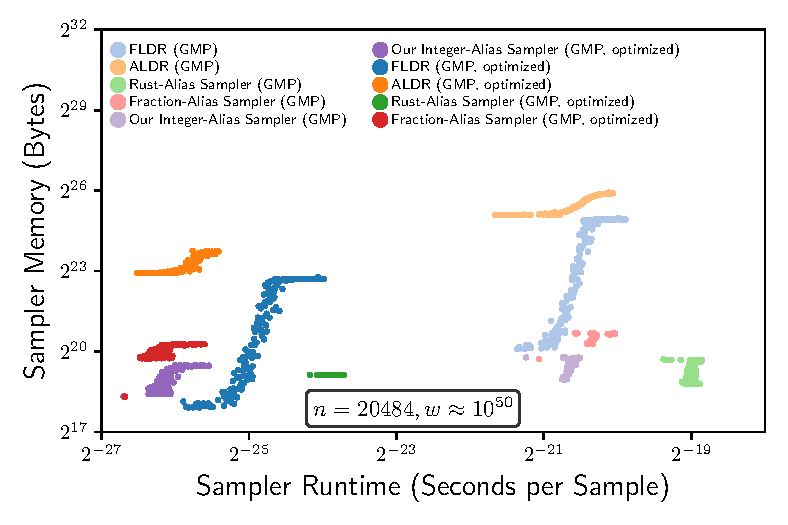
\includegraphics[width=\linewidth]{figures/figure-4-interpolation-runtime-memory.pdf}
  \caption{Temps et mémoire.}
\end{subfigure}\hfill
\begin{subfigure}{0.49\textwidth}
  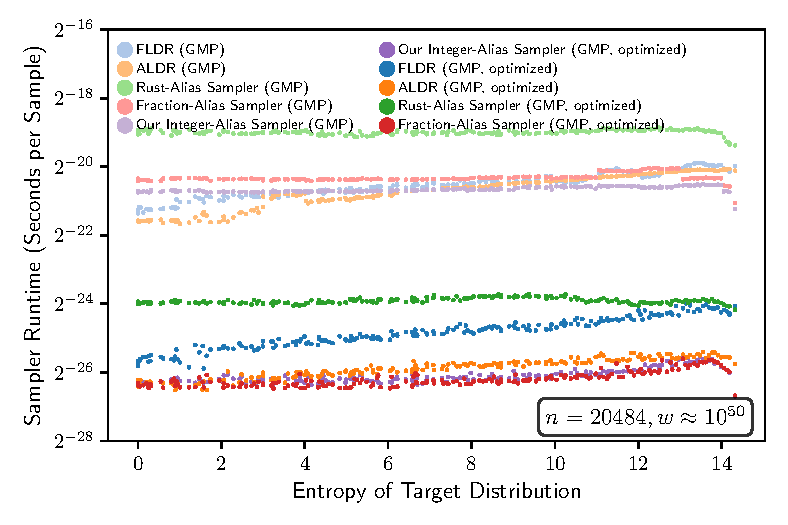
\includegraphics[width=\linewidth]{figures/figure-4-interpolation-entropy-runtimes.pdf}
  \caption{Temps en fonction de l'entropie.}
\end{subfigure}

\vspace{1em}
\begin{subfigure}{0.49\textwidth}
  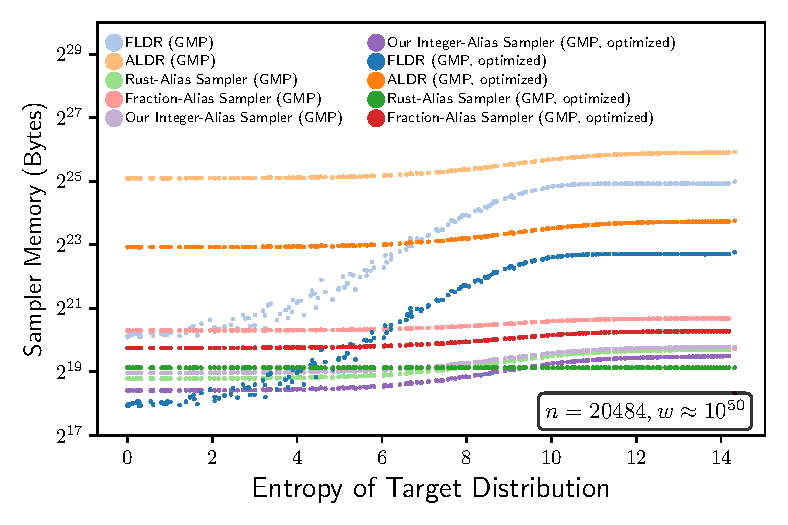
\includegraphics[width=\linewidth]{figures/figure-4-interpolation-entropy-memory.pdf}
  \caption{Mémoire en fonction de l'entropie.}
\end{subfigure}\hfill
\begin{subfigure}{0.49\textwidth}
  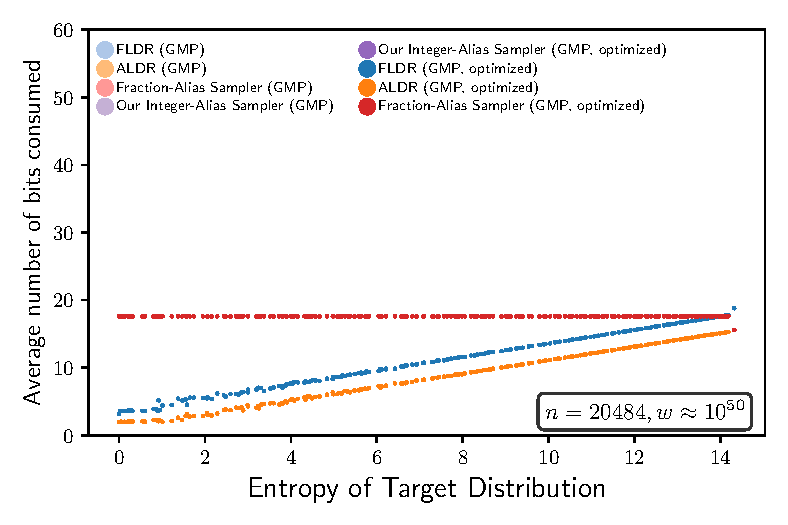
\includegraphics[width=\linewidth]{figures/figure-4-interpolation-entropy-bits.pdf}
  \caption{Bits consommés en fonction de l'entropie.}
\end{subfigure}
\caption{Figures du notebook \code{figure-4-interpolation\_Antoine.ipynb}. Chaque
algorithme a sa teinte : clair pour l'original, foncé pour la version optimisée. Sur
la figure~(d), les points des versions optimisées recouvrent ceux des originaux
(consommation identique) ; Rust-Alias (185 bits) est hors échelle.}
\label{fig:resultats}
\end{figure}

\begin{figure}[p]
\centering
\begin{subfigure}{0.49\textwidth}
  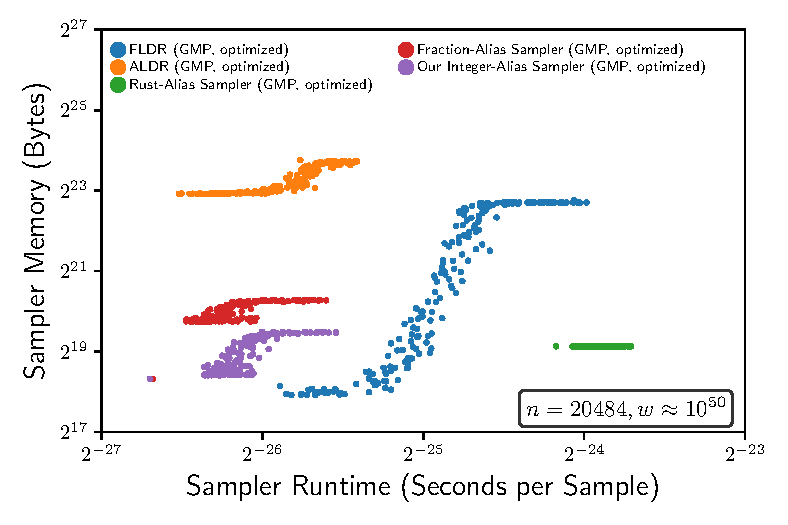
\includegraphics[width=\linewidth]{figures/opt-runtime-memory.pdf}
  \caption{Temps et mémoire.}
\end{subfigure}\hfill
\begin{subfigure}{0.49\textwidth}
  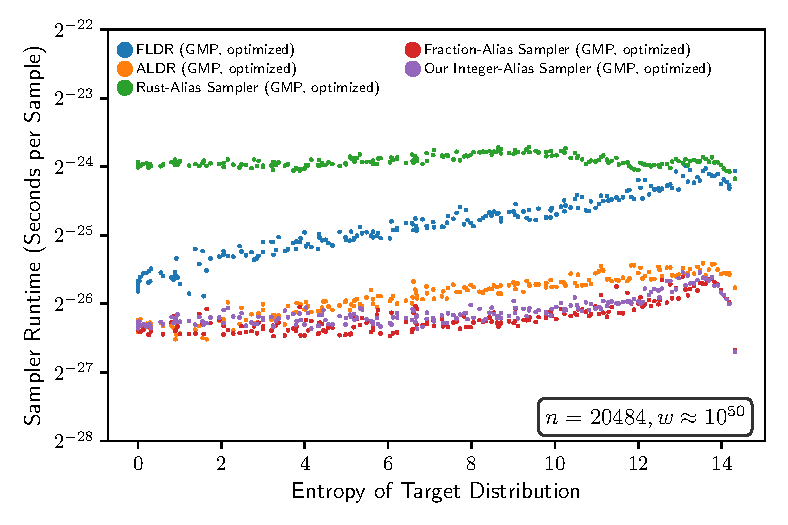
\includegraphics[width=\linewidth]{figures/opt-entropy-runtimes.pdf}
  \caption{Temps en fonction de l'entropie.}
\end{subfigure}

\vspace{1em}
\begin{subfigure}{0.49\textwidth}
  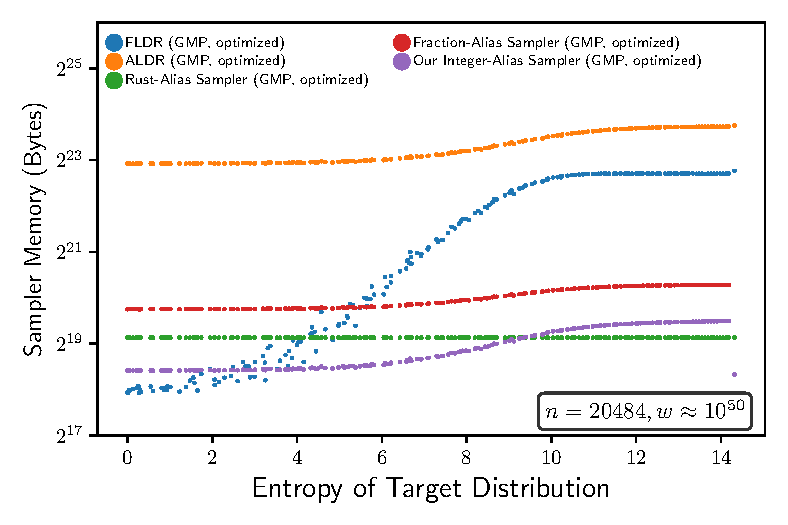
\includegraphics[width=\linewidth]{figures/opt-entropy-memory.pdf}
  \caption{Mémoire en fonction de l'entropie.}
\end{subfigure}\hfill
\begin{subfigure}{0.49\textwidth}
  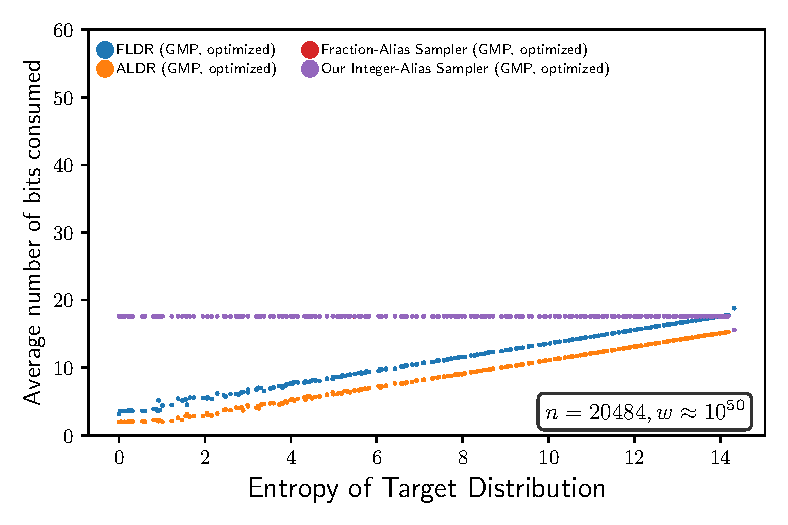
\includegraphics[width=\linewidth]{figures/opt-entropy-bits.pdf}
  \caption{Bits consommés en fonction de l'entropie.}
\end{subfigure}
\caption{Mêmes mesures que la figure~\ref{fig:resultats}, avec les seules versions
optimisées et des axes resserrés, pour les comparer entre elles. Les couleurs sont
celles de la figure~\ref{fig:resultats}. Sur la figure~(d), Rust-Alias (185 bits) est
hors échelle.}
\label{fig:opt}
\end{figure}

\subsection{Temps}

Toutes les versions optimisées sont plus rapides que tous les originaux, sur toute la
plage d'entropie (figure~\ref{fig:resultats}b). Parmi elles (figure~\ref{fig:opt}), Integer-Alias,
Fraction-Alias et ALDR sont les plus rapides (10 à 22~ns par tirage), suivis de FLDR
(16 à 60~ns) puis de Rust-Alias (53 à 73~ns), qui paie son uniforme de 185 bits. Les
méthodes Alias gardent un temps quasi constant ; FLDR et ALDR croissent avec
l'entropie, comme leurs originaux.

Exécutés seuls (sans la charge du pipeline), les gains sont du même ordre :

\begin{table}[H]
\centering
\small
\begin{tabular}{lrrr}
\toprule
$10^7$ tirages, exécution seule & \code{d.00000} & \code{d.00100} & \code{d.00180} \\
\midrule
Integer-Alias  & 3,79 s $\to$ 0,10 s & 4,09 s $\to$ 0,10 s & 4,25 s $\to$ 0,14 s \\
FLDR (corrigé) & 3,20 s $\to$ 0,16 s & 4,02 s $\to$ 0,30 s & 5,98 s $\to$ 0,45 s \\
ALDR           & 3,38 s $\to$ 0,11 s & 6,10 s $\to$ 0,15 s & 8,35 s $\to$ 0,18 s \\
Rust-Alias     & 8,64 s $\to$ 0,48 s & 8,58 s $\to$ 0,51 s & 8,72 s $\to$ 0,51 s \\
Fraction-Alias & 4,62 s $\to$ 0,10 s & 5,01 s $\to$ 0,10 s & 5,10 s $\to$ 0,14 s \\
\bottomrule
\end{tabular}
\end{table}

\paragraph{Variabilité entre sessions.} Les temps des originaux mesurés ce jour
diffèrent de ceux de la série précédente de $-21$ à $+8\,\%$ (par exemple
Integer-Alias : 616~ns puis 594~ns ; Rust-Alias : 1774~ns puis 1918~ns). C'est l'ordre
de grandeur de la variabilité due aux conditions de la machine ; elle ne change pas
les conclusions.

\subsection{Mémoire}

FLDR et ALDR passent d'entiers \code{mpz\_t} (16 octets d'en-tête plus les limbs) à des
entiers 32 bits : $-78\,\%$ chacun. Integer-Alias ($-28\,\%$) et Fraction-Alias
($-30\,\%$) gagnent grâce aux seuils stockés en octets, uniquement pour les cellules
avec alias. Rust-Alias augmente de 9\,\% (voir plus haut). Integer-Alias optimisé reste
l'échantillonneur le plus compact de la comparaison.

\subsection{Bits aléatoires}

La consommation de chaque version optimisée est égale à celle de son original
(Integer-Alias 17,59 ; FLDR corrigé 10,66 ; ALDR 8,29 ; Rust-Alias 185,20 ;
Fraction-Alias 17,59 bits par tirage). Les analyses de l'article (proposition~4,
lemme~3) s'appliquent donc sans changement, à ceci près que les valeurs de FLDR
doivent être reprises après correction.

\section{Mesures séquentielles des versions optimisées}
\label{sec:sequentiel}

Pour supprimer la contention décrite en section~\ref{sec:pipeline}, les cinq versions
optimisées ont été remesurées avec la version séquentielle du pipeline
(\code{experiments/pipeline\_seq.sh}), avec en plus \code{alias.integers\_v2}
(section~\ref{sec:v2}). Le protocole est celui de la figure~4 :
201 distributions de \code{distributions\_entropy}, $10^7$ tirages par distribution,
temps \code{clock()}. Mais une seule mesure tourne à la fois, chaque échantillonneur est
mesuré une fois, et les six échantillonneurs sont mesurés à la suite pour chaque
distribution. L'exécution complète prend environ 9 minutes sur le M4 Pro. Les figures
sont produites par \code{figure-4-interpolation\_Antoine.ipynb}, restreint à ces six
échantillonneurs (fichiers \code{figure-4-interpolation-opt-*}).

\begin{table}[H]
\centering
\small
\begin{tabular}{lrrr}
\toprule
Temps par tirage (ns) & Pipeline parallèle (médiane) & Séquentiel (médiane) & Séquentiel (min--max) \\
\midrule
Integer-Alias  & 13,3 & 10,5 & 8,5--17,3 \\
FLDR           & 33,6 & 28,3 & 14,4--51,4 \\
ALDR           & 16,6 & 14,1 & 9,2--20,3 \\
Rust-Alias     & 62,6 & 50,4 & 44,5--57,0 \\
Fraction-Alias & 12,4 & 10,1 & 8,1--16,6 \\
\midrule
Integer-Alias v2 & -- & 4,4 & 4,1--7,1 \\
\bottomrule
\end{tabular}
\caption{Versions optimisées et v2, 201 distributions, série du 22 octobre. La colonne
« pipeline parallèle » reprend la table~\ref{tab:resume} ; v2 n'y a pas été mesuré.}
\end{table}

\noindent Sans contention, les temps baissent de 15 à 21\,\% (en médiane), et le
classement des cinq versions optimisées ne change pas. Integer-Alias et Fraction-Alias
sont les plus rapides et presque constants en fonction de l'entropie ; viennent ensuite
ALDR, puis FLDR, qui croît nettement avec l'entropie, puis Rust-Alias. Integer-Alias v2
est le plus rapide de tous, sur toute la plage d'entropie : 4,4~ns en médiane, 2,3 fois
moins qu'Integer-Alias (section~\ref{sec:v2}). La mémoire et les bits ne dépendent
pas du mode d'exécution : ils sont identiques à ceux de la section précédente. Les
originaux (\code{\_gmp}) n'ont pas été remesurés en séquentiel. Les gains de la
table~\ref{tab:resume} restent donc ceux du pipeline parallèle, où les deux versions
sont mesurées dans les mêmes conditions.

\paragraph{Pourquoi Integer-Alias dépasse Rust-Alias en mémoire vers $H \approx 10$.}
Sur la figure~\ref{fig:sequentiel}c, la courbe d'Integer-Alias passe au-dessus de celle
de Rust-Alias vers une entropie de 10. La raison tient à la façon dont chacun stocke ses
seuils.
\begin{itemize}
\item \textbf{Rust-Alias} stocke chaque seuil à largeur fixe, celle de $W$ : 3 limbs de
  8 octets. Avec l'alias (4 octets), cela fait 28 octets par objet, soit
  $28 \times 20\,484 \approx 574$~Ko pour toutes les distributions. Sa courbe est plate.
\item \textbf{Integer-Alias} stocke des cellules de 16 octets ($16 \times 20\,485
  \approx 328$~Ko), plus chaque seuil exact $T_i$ avec ses seuls octets utiles, et
  seulement pour les cellules avec alias. À basse entropie, les petits objets ont des
  poids minuscules (beaucoup valent 1) : chaque seuil tient sur environ 1 octet, et le
  total reste vers 350~Ko. Quand l'entropie monte, les poids des petits objets se
  rapprochent de $\cs \approx 2\cdot 10^{46}$, soit environ 20 octets par seuil : le
  total atteint 720~Ko.
\end{itemize}
Les deux courbes se croisent quand les seuils d'Integer-Alias dépassent en moyenne
environ $(574 - 328)/20\,485 \approx 12$ octets, ce qui arrive vers $H \approx 10$.
Le dernier point, la distribution uniforme, retombe à 328~Ko : aucune cellule n'a
d'alias, donc il n'y a aucun seuil à stocker.

\begin{figure}[H]
\centering
\begin{subfigure}{0.49\textwidth}
  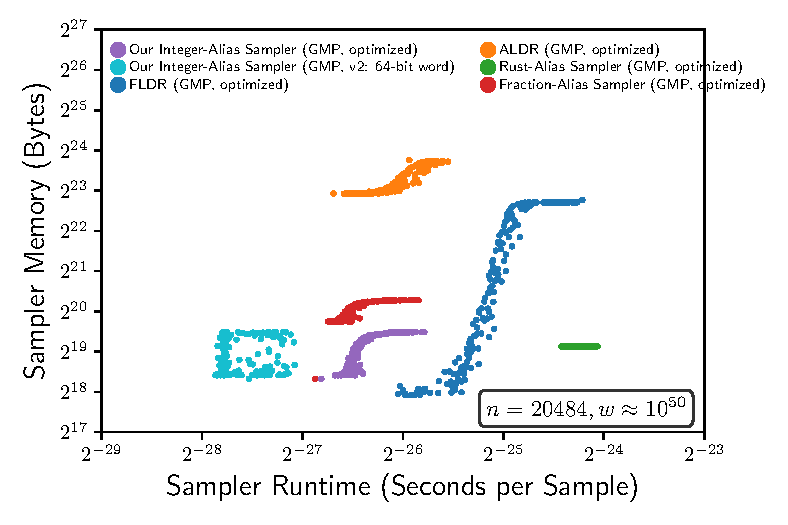
\includegraphics[width=\linewidth]{figures/seq-opt-runtime-memory.pdf}
  \caption{Temps et mémoire.}
\end{subfigure}\hfill
\begin{subfigure}{0.49\textwidth}
  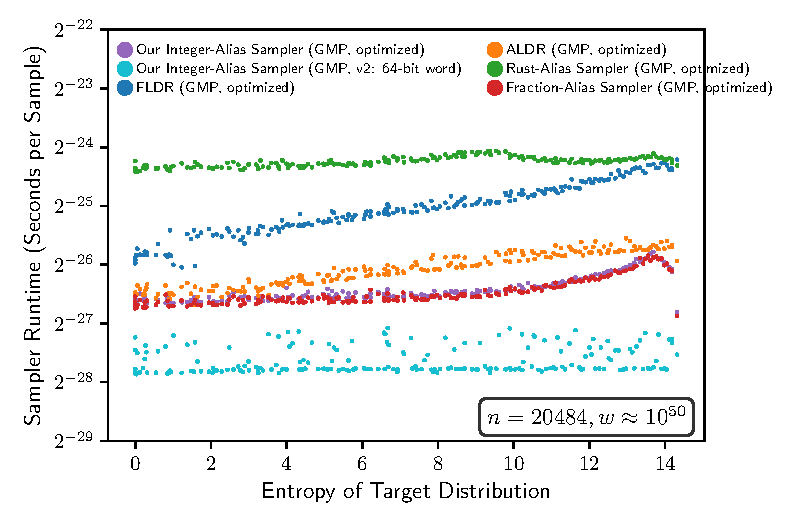
\includegraphics[width=\linewidth]{figures/seq-opt-entropy-runtimes.pdf}
  \caption{Temps en fonction de l'entropie.}
\end{subfigure}

\vspace{1em}
\begin{subfigure}{0.49\textwidth}
  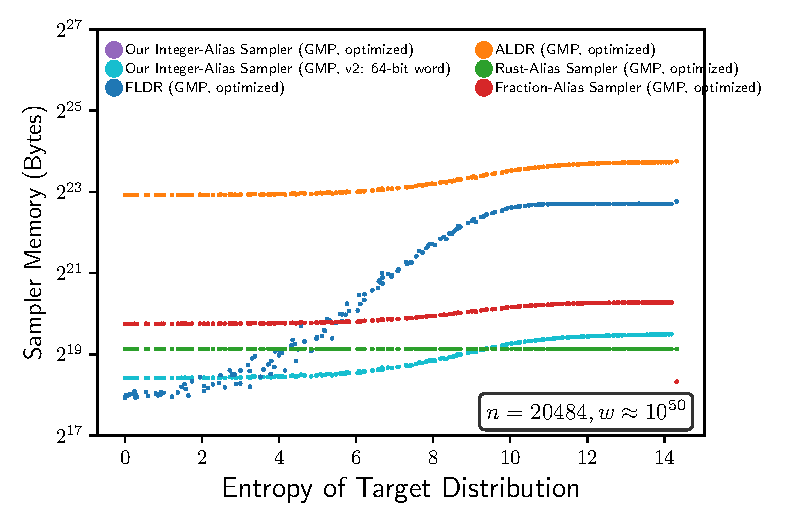
\includegraphics[width=\linewidth]{figures/seq-opt-entropy-memory.pdf}
  \caption{Mémoire en fonction de l'entropie.}
\end{subfigure}\hfill
\begin{subfigure}{0.49\textwidth}
  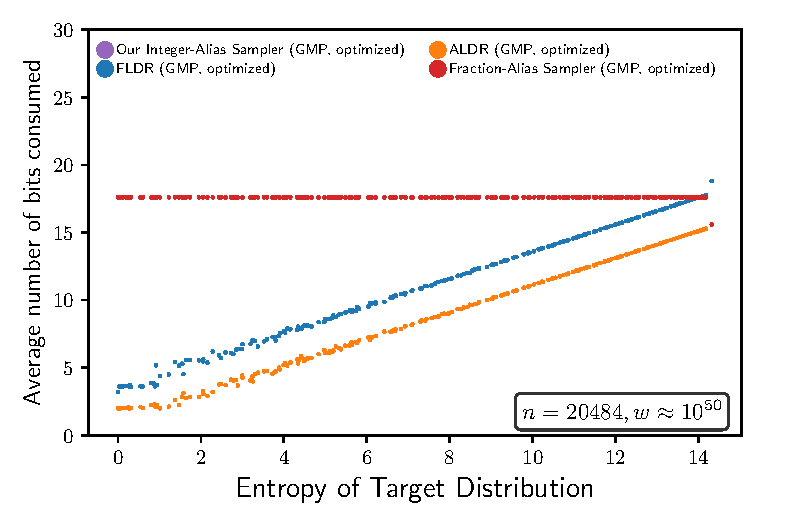
\includegraphics[width=\linewidth]{figures/seq-opt-entropy-bits.pdf}
  \caption{Bits consommés en fonction de l'entropie.}
\end{subfigure}
\caption{Versions optimisées et Integer-Alias v2 (en cyan), pipeline séquentiel
(\code{pipeline\_seq.sh}). Sur la figure~(c), v2 a la même mémoire qu'Integer-Alias
et leurs points se recouvrent. Sur la figure~(d), Integer-Alias et Fraction-Alias
consomment le même nombre de bits et leurs points se recouvrent ; Rust-Alias
(185 bits) et v2 (64 bits) sont hors échelle (voir la figure~\ref{fig:sequentiel-bits}).}
\label{fig:sequentiel}
\end{figure}

\begin{figure}[H]
\centering
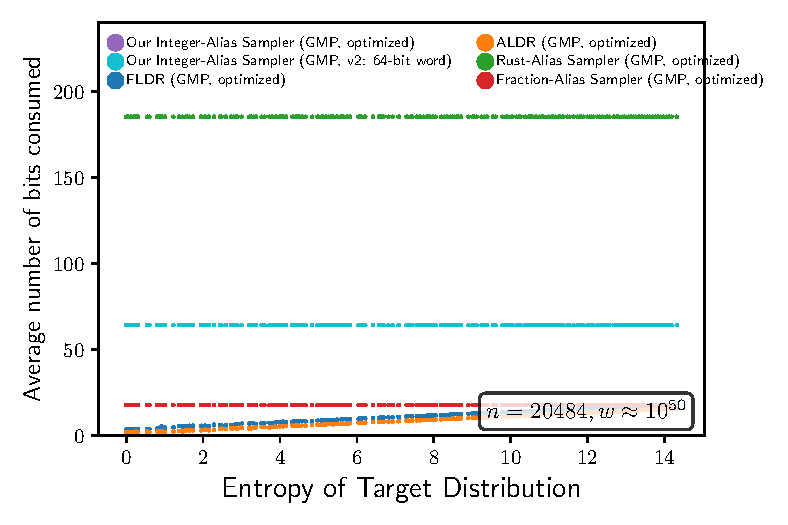
\includegraphics[width=0.6\textwidth]{figures/seq-opt-entropy-bits-rust.pdf}
\caption{Bits consommés, échelle complète : Rust-Alias (185 bits), Integer-Alias v2
(64 bits), puis les autres versions optimisées, entre 2 et 19 bits.}
\label{fig:sequentiel-bits}
\end{figure}

\subsection{Temps de preprocessing}
\label{sec:preprocessing}

\paragraph{Mesure.} Le programme \code{c/measure\_preprocess.c} lit d'abord les poids,
sans chronométrer cette lecture, puis mesure la seule construction de la structure de
tirage à partir des poids. Il la répète au moins 5 fois et pendant au moins 50~ms, et
garde le meilleur temps (horloge \code{CLOCK\_MONOTONIC\_RAW}). La construction est celle
qu'utilise chaque échantillonneur :
\code{preprocess\_alias\_integers\_opt}, \code{preprocess\_alias\_integers\_v2} (la même,
plus le calcul des 32 chiffres $D_i$), \code{preprocess\_aldr\_opt}, et pour Rust-Alias
et Fraction-Alias la construction d'origine suivie de la conversion vers la table
optimisée. La commande \code{./pipeline\_seq.sh distributions\_entropy
measure-preprocess} (aussi lancée par \code{run-all}) écrit un fichier
\code{<sampler>.preprocess} par échantillonneur ; elle prend environ 2 minutes.

\paragraph{FLDR porté en C.} L'arbre DDG de FLDR était construit en Python
(\code{src/rejection.py}, \code{matrix.py}, \code{tree.py}, \code{packing.py}), et le C
ne faisait que relire l'encodage. Pour comparer des temps C entre eux, nous avons écrit
\code{preprocess\_fldr\_opt} (\code{c/fldr\_opt.c}). Comme la matrice de FLDR est
dyadique ($\sum_i M_i = 2^k$), l'arbre n'a pas d'arête de retour, et il se décrit
profondeur par profondeur. À la profondeur $d$, les enfants des nœuds internes de la
profondeur $d-1$ sont, de gauche à droite, les nœuds internes, puis les feuilles des
lignes dont le bit $k-d$ vaut 1, par ligne décroissante. L'encodage est ensuite écrit
en préordre, comme \code{pack\_tree}. On évite ainsi les indices de nœuds de
$k \approx 170$ bits de la version Python. Sur les 201 distributions, l'encodage produit
est \emph{identique} à celui des fichiers \code{.rej.enc\_opt} écrits par Python
(\code{measure\_preprocess.out.opt check-fldr}).

\paragraph{Une particularité des données.} Pour la distribution uniforme
(\code{d.00200}), la somme des poids dépasse de $1{,}25\cdot 10^{34}$ (soit
$2{,}7\cdot 10^{-17}$ en relatif) le $Z$ écrit en première ligne du fichier, à cause de
l'arrondi de \code{normalize\_to\_Z}. Les méthodes Alias et ALDR normalisent par la
somme des poids, et tirent bien l'uniforme. FLDR utilise les probabilités $w_i/Z$ :
il tire aussi l'uniforme, grâce au rejet, mais avec $k = 169$ au lieu de 15 et un arbre
plus grand. Le portage en C reprend cette convention, pour rester identique à Python.

\begin{figure}[H]
\centering
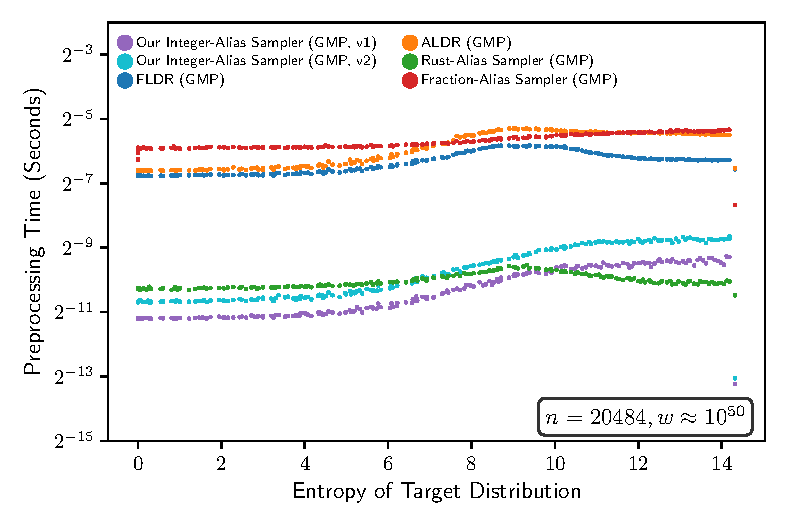
\includegraphics[width=0.75\textwidth]{figures/seq-opt-entropy-preprocess.pdf}
\caption{Temps de construction de la structure à partir des poids, en fonction de
l'entropie (201 distributions, $n = 20\,484$). Integer-Alias v1 est
\code{alias.integers\_opt}.}
\label{fig:preprocessing}
\end{figure}

\begin{table}[H]
\centering
\small
\begin{tabular}{lrrr}
\toprule
Construction (ms) & Médiane & Min & Max \\
\midrule
Integer-Alias (\code{opt})   & 0,68  & 0,10 & 1,62 \\
Integer-Alias v2             & 1,03  & 0,12 & 2,49 \\
Rust-Alias                   & 0,93  & 0,70 & 1,35 \\
FLDR                         & 12,85 & 9,15 & 17,72 \\
ALDR                         & 17,04 & 10,22 & 25,58 \\
Fraction-Alias               & 18,34 & 4,88 & 24,84 \\
\bottomrule
\end{tabular}
\end{table}

\begin{itemize}
\item \textbf{Integer-Alias est la construction la plus rapide} : de 0,1 à 1,6~ms, soit
  en médiane 19 à 27 fois moins que FLDR, ALDR et Fraction-Alias. Sur les mêmes distributions, la
  construction d'origine (\code{preprocess\_gmp\_alias\_integers}) prend environ 1~ms.
  La version optimisée est donc du même ordre : elle ajoute une division GMP par cellule
  pour les 31 chiffres du seuil, mais range les seuils en octets.
\item \textbf{Elle croît avec l'entropie}, entre $H \approx 6$ et $H \approx 10$, pour
  la même raison que sa mémoire (section~\ref{sec:sequentiel}) : les seuils $T_i$ des
  petits objets passent d'environ 1 octet à environ 20, et la division GMP qui calcule
  leurs chiffres coûte plus cher. La distribution uniforme n'a aucune cellule avec alias :
  0,1~ms.
\item \textbf{v2 coûte environ 50\,\% de plus qu'\code{opt}} : il construit la table
  d'\code{opt}, puis fait une seconde division GMP par cellule pour les 32 chiffres $D_i$.
  On pourrait calculer $D_i$ directement, avec une seule division ; nous ne l'avons pas
  fait, car le preprocessing reste sous 2,5~ms.
\item \textbf{Rust-Alias} est presque constant (environ 1~ms) : sa construction ne
  multiplie les poids que par $n$, sans division par cellule.
\item \textbf{FLDR et ALDR} parcourent les bits de chaque ligne à chaque profondeur :
  $k \approx 170$ niveaux pour FLDR et $K = 2k \approx 340$ pour ALDR, sur
  $n \approx 20\,000$ lignes. Leur coût suit le nombre de feuilles, qui croît avec
  l'entropie.
\item \textbf{Fraction-Alias} manipule des rationnels GMP (\code{mpq\_t}), qui sont
  normalisés par un calcul de pgcd après chaque opération : c'est la construction la
  plus lente.
\end{itemize}

\section{Peut-on faire mieux pour l'uniforme et le Bernoulli ?}
\label{sec:optimalite}

Un tirage d'Integer-Alias se compose d'une uniforme sur les $q$ cellules (Fast Dice
Roller, FDR) et d'un Bernoulli($T_i/\cs$) (algorithme de Lumbroso, ici avec chiffres
précalculés). Ces deux briques sont-elles optimales en nombre de bits, et le sont-elles
aussi en temps ? Les mesures de cette section sont faites avec
\code{rapport\_optimisation/bench\_temps/bench.c} ; les calculs exacts avec
\code{theory.py}, les tests avec \code{chi2.py}, dans le même dossier.

\subsection{En bits : optimales pour un tirage isolé}

Le théorème de Knuth et Yao (1976) dit que tout algorithme qui tire un objet de loi $p$
à partir de bits frais en consomme en moyenne au moins $H(p)$, et que l'arbre de
Knuth--Yao (KY) atteint le minimum, compris entre $H(p)$ et $H(p)+2$.

\paragraph{Uniforme.} Nous avons calculé exactement le nombre moyen de bits du FDR (en
suivant la chaîne des états de la boucle) et celui de l'arbre KY de l'uniforme sur
$[0, n)$ (à partir des chiffres binaires de $1/n$) :
\begin{table}[H]
\centering
\small
\begin{tabular}{rrrr}
\toprule
$n$ & $\log_2 n$ & FDR & KY \\
\midrule
3 & 1,585 & 2,667 & 2,667 \\
7 & 2,807 & 3,429 & 3,429 \\
1\,000 & 9,966 & 10,151 & 10,151 \\
16\,385 & 14,000 & 15,999 & 15,999 \\
20\,485 & 14,322 & 15,597 & 15,597 \\
\bottomrule
\end{tabular}
\end{table}
\noindent Les deux coïncident pour toutes les valeurs testées (11 valeurs de $n$, de 3
à 24\,576) : aucun algorithme qui tire une uniforme isolée ne consomme moins de bits que
le FDR. Sur la table du protocole ($q = 20\,485$), il perd 1,27 bit par rapport à
$\log_2 q$, et cette perte est inévitable pour un tirage isolé.

\paragraph{Bernoulli.} Si $p$ n'est pas dyadique, les développements binaires de $p$ et
de $1-p$ sont complémentaires : l'arbre KY de Bernoulli($p$) a exactement une feuille à
chaque profondeur, et coûte $\sum_k k\,2^{-k} = 2$ bits. Le Bernoulli de Lumbroso est
précisément cet arbre (pièce $k$ égale à 1 : feuille de profondeur $k$, étiquette $d_k$).
Si $p$ est dyadique, les deux s'arrêtent au dernier chiffre. Le Bernoulli est donc
optimal pour un tirage isolé.

\paragraph{Mais pas pour une suite de tirages.} Ces bornes portent sur \emph{un} tirage
qui part de bits frais. Quand on tire une suite d'objets, les bits « inutilisés » par un
tirage peuvent servir au suivant, et la borne devient $H$ par tirage. Pour la structure
d'Integer-Alias, le minimum est alors l'entropie du couple (cellule, résultat du
Bernoulli), $\log_2 q + \mathbb{E}_i[h(T_i/\cs)]$, où $h$ est l'entropie binaire. Sur
les distributions du protocole, les seuils sont presque tous très proches de 0 (petits
objets de poids $\ll \cs$) : $\mathbb{E}[h] = 0{,}022$ bit sur \code{d.00100}, alors que
le Bernoulli en dépense 2. Integer-Alias consomme 17,60 bits là où 14,34 suffisent pour
la même table.

\subsection{En temps : pas optimales}

Il n'existe pas de borne inférieure théorique utile en temps : dans le modèle RAM
avec des mots de 64 bits, un tirage coûte $\Omega(1)$ opérations, plus la lecture d'environ
$H/64$ mots aléatoires. La question porte donc sur les constantes, et nous l'avons
traitée par la mesure.

\paragraph{Variantes comparées.} Toutes utilisent la même table (celle
d'\code{alias.integers\_opt}) et le même flux de bits (\code{flip\_opt}).
\begin{itemize}
\item \textbf{Lemire} (2019) : uniforme par multiplication d'un mot de 64 bits par $q$,
  rejet de probabilité $< q/2^{64}$. Exacte, mais 64 bits par tirage.
\item \textbf{Recyclage} : on garde d'un tirage à l'autre un état $(U, M)$, avec $U$
  uniforme sur $[0, M)$ ; quand $M < 2^{32}$, on ajoute 32 bits frais
  ($U \leftarrow 2^{32}U + B$, $M \leftarrow 2^{32}M$). C'est le principe du codage
  arithmétique et de l'algorithme d'intervalle de Han et Hoshi (1997).
  \begin{itemize}
  \item Uniforme sur $[0, q)$ : on écrit $M = aq + r$. Si $U < aq$, on renvoie
    $U \bmod q$ et l'état devient $(\lfloor U/q \rfloor, a)$ ; sinon l'état devient
    $(U - aq, r)$ et on recommence. La seule information perdue est le choix entre ces
    deux branches.
  \item Bernoulli($p$), $p = T_i/\cs$ : on précalcule $P = \lfloor p\,2^{64} \rfloor$
    (8 octets par cellule) et $\ell = \lfloor P M / 2^{64} \rfloor$ (une
    multiplication). Si $U < \ell$, on renvoie 1 et l'état devient $(U, \ell)$ ; si
    $U \ge \ell + 2$, on renvoie 0 et l'état devient $(U - \ell - 2, M - \ell - 2)$.
    Le cas restant (probabilité $\le 2/M \le 2^{-31}$) est tranché exactement en GMP
    avec des bits frais, puis l'état est abandonné.
  \end{itemize}
\item \textbf{cmp31} : Bernoulli par comparaison de 31 bits frais avec les 31 chiffres
  d'un coup (exact, 31 bits par appel).
\item \textbf{Plancher inexact} : un mot de 64 bits, 32 bits pour la cellule et 32 bits
  comparés à un seuil arrondi. Ce n'est pas exact (biais de l'ordre de $2^{-32}$), mais
  c'est à peu près ce que coûte au minimum une méthode Alias avec ce flux de bits.
\end{itemize}

\paragraph{Exactitude du recyclage.} Par récurrence, sachant tout le passé, $U$ est
uniforme sur $[0, M)$. Le remplissage conserve cette propriété. Dans l'uniforme,
conditionnellement à $U < aq$, le couple $(U \bmod q, \lfloor U/q \rfloor)$ est
uniforme sur $[0,q) \times [0,a)$ : le résultat est uniforme et indépendant du nouvel
état. Dans le Bernoulli, soit $V = (U + \Theta)/M$ avec $\Theta$ uniforme sur $[0,1)$
(jamais tirée) : $V$ est uniforme sur $[0, 1)$, et le résultat vaut exactement
$\mathbf{1}\{V < p\}$, car $U < \ell$ entraîne $V < p$ et $U \ge \ell+2$ entraîne
$V \ge p$. Dans chaque branche, le nouvel état est uniforme sur son intervalle. Les
tirages successifs sont donc indépendants et de loi exacte. Vérification : $\chi^2$ sur
$5\cdot 10^7$ tirages de \code{d.00100}, $p = 0{,}82$ ; test des paires successives
(classes de masse $\approx 1/8$), $p = 0{,}80$. Les autres variantes exactes donnent des
p-valeurs de 0,13 à 0,91.

\paragraph{Mesures.} MacBook Pro M4 Pro, un seul processus, $2\cdot 10^7$ tirages,
meilleur de trois essais. On donne le temps réel par tirage, le temps CPU entre
parenthèses (\code{clock()}, producteur compris, comme dans le pipeline) et les bits
consommés.

\begin{table}[H]
\centering
\small
\begin{tabular}{lrrr}
\toprule
Brique seule (\code{d.00100}) & Temps (ns) & (CPU) & Bits \\
\midrule
Uniforme FDR (actuelle)  & 6,93 & (7,54) & 15,60 \\
Uniforme Lemire          & 3,46 & (5,21) & 64,00 \\
Uniforme recyclage       & 5,57 & (6,11) & 14,32 \\
\midrule
Bernoulli à chiffres, \code{ctz} (actuel) & 2,88 & (3,02) & 2,00 \\
Bernoulli recyclage      & 2,91 & (2,99) & 0,02 \\
Bernoulli cmp31          & 3,90 & (4,78) & 31,00 \\
\midrule
Lecture de 18 bits du flux & 2,76 & (3,31) & 18,00 \\
Lecture d'une cellule au hasard & 1,58 & (1,63) & -- \\
\bottomrule
\end{tabular}
\end{table}

\begin{table}[H]
\centering
\small
\setlength{\tabcolsep}{4pt}
\begin{tabular}{lrrrrrr}
\toprule
Tirage complet & Bits & \code{d.00000} & \code{d.00050} & \code{d.00100} & \code{d.00150} & \code{d.00200} \\
Entropie $H(p)$ & & 0,00 & 3,73 & 7,08 & 10,74 & 14,32 \\
\midrule
\multicolumn{7}{l}{\emph{Temps réel (ns par tirage)}} \\
FDR + \code{ctz} (actuel)  & 17,6$^*$ & 9,30 & 9,48 & 9,68 & 11,18 & 8,26 \\
Lemire + \code{ctz}        & 66,0$^*$ & 6,14 & 6,19 & 6,51 & 7,74 & 4,18 \\
Recyclage + \code{ctz}     & 16,3$^*$ & 5,81 & 6,02 & 6,50 & 7,83 & 4,97 \\
Recyclage, 1 état          & 14,3--14,5 & 8,37 & 11,23 & 13,16 & 13,68 & 5,04 \\
\textbf{Recyclage, 2 états} & 14,3--14,5 & \textbf{4,89} & \textbf{5,13} & \textbf{5,40} & \textbf{7,19} & \textbf{5,04} \\
Plancher inexact           & 64,0 & 4,14 & 4,20 & 4,32 & 4,39 & 4,47 \\
\midrule
\multicolumn{7}{l}{\emph{Temps CPU (ns par tirage, producteur compris)}} \\
FDR + \code{ctz} (actuel)  & & 10,0 & 10,1 & 10,4 & 12,0 & 8,9 \\
Recyclage, 2 états         & & 5,4 & 5,7 & 6,0 & 7,8 & 5,6 \\
Plancher inexact           & & 5,9 & 6,0 & 6,1 & 6,2 & 6,3 \\
\bottomrule
\end{tabular}
\caption{\code{ctz} : Bernoulli à chiffres précalculés actuel. $^*$Sur \code{d.00200}, 2 bits de moins
(15,6 ; 64,0 ; 14,3) : c'est la distribution uniforme, $q = n$ et aucune cellule n'a
d'alias, il n'y a donc pas de Bernoulli. Les écarts entre deux exécutions sont de
l'ordre de 0,3~ns.}
\label{tab:variantes}
\end{table}

\paragraph{Lecture des résultats.}
\begin{enumerate}
\item \textbf{L'uniforme FDR est le poste le plus coûteux} : environ 7~ns, deux fois
  Lemire. Après le premier bloc de $\lceil \log_2 q \rceil$ bits, la boucle lit un bit
  par itération, et sa sortie dépend du hasard : pour $q = 20\,485$, le premier bloc est
  accepté avec probabilité $20\,485/2^{15} \approx 0{,}63$ seulement. Les erreurs de
  prédiction de branchement qui en résultent en sont la cause probable ; nous n'avons
  pas pu lire les compteurs matériels sous macOS pour le confirmer.
\item \textbf{Le Bernoulli à chiffres précalculés est déjà au coût de la lecture de ses
  bits} (2,4 à 2,9~ns, contre 2,7~ns pour lire 18 bits du flux) : pas de boucle, un
  \code{ctz} et un décalage. La comparaison directe sur 31 bits (cmp31) est plus lente
  et consomme 15 fois plus de bits : ici, économiser les bits ne coûte pas de temps. Le
  Bernoulli recyclé prend le même temps pour 0,02 bit au lieu de 2. Sur \code{d.00150},
  où les seuils sont moins extrêmes ($\mathbb{E}[h] = 0{,}18$), le résultat du Bernoulli
  devient moins prévisible et toutes les variantes ralentissent.
\item \textbf{Le recyclage avec deux états} est 1,8 fois plus rapide que la version
  actuelle sur \code{d.00100} (5,40 contre 9,68~ns) et consomme 3,3 bits de moins
  (14,34 contre 17,60). En temps réel, il est à 1~ns du plancher inexact ; en temps CPU,
  il est en dessous du plancher sauf sur \code{d.00150}, car il demande 4,5 fois moins
  de bits au producteur. Avec un seul état partagé, il est au contraire plus lent : le Bernoulli
  lit $P_i$ en mémoire, et l'uniforme suivante attend l'état mis à jour par ce
  Bernoulli. La latence mémoire entre alors dans la chaîne de dépendances d'un tirage
  au suivant. Avec deux états, la chaîne de l'uniforme n'attend plus cette lecture, et
  le processeur recouvre les tirages successifs.
\end{enumerate}

\subsection{Remplacer les algorithmes de Lumbroso, au prix de bits}

On peut aussi échanger des bits contre du temps, sans recyclage, en remplaçant chaque
brique par un algorithme exact plus simple. Deux variantes de plus :
\begin{itemize}
\item \textbf{Lemire32} : uniforme de Lemire sur un mot de 32 bits (rejet de
  probabilité $< q/2^{32} \approx 5\cdot 10^{-6}$), suivie du Bernoulli actuel.
\item \textbf{Mot de 64 bits exact} : la version exacte du plancher. Les 32 bits de
  poids fort donnent la cellule (Lemire32), et les 32 bits de poids faible sont comparés
  aux 32 premiers chiffres de $T_i/\cs$. En cas d'égalité (probabilité $2^{-32}$), la
  suite est tirée exactement en GMP.
\end{itemize}

\begin{table}[H]
\centering
\small
\setlength{\tabcolsep}{4pt}
\begin{tabular}{lrrrr}
\toprule
Temps (ns) / bits & \code{d.00000} & \code{d.00100} & \code{d.00150} & \code{d.00200} \\
\midrule
FDR + Bernoulli \code{ctz} (actuel) & 8,96 / 17,6 & 9,35 / 17,6 & 10,54 / 17,6 & 7,70 / 15,6 \\
Lemire 64 + Bernoulli \code{ctz}    & 5,73 / 66,0 & 6,33 / 66,0 & 7,28 / 66,0 & 3,87 / 64,0 \\
Lemire32 + Bernoulli \code{ctz}     & 5,54 / 34,0 & 5,98 / 34,0 & 6,80 / 34,0 & 3,34 / 32,0 \\
\textbf{Mot de 64 bits exact}       & \textbf{4,08} / 64,0 & \textbf{4,39} / 64,0 & \textbf{4,54} / 64,0 & 3,95 / 64,0 \\
Recyclage, 2 états                  & 4,80 / 14,3 & 5,11 / 14,3 & 6,90 / 14,5 & 4,88 / 14,3 \\
Plancher inexact                    & 3,91 / 64,0 & 4,34 / 64,0 & 4,23 / 64,0 & 4,47 / 64,0 \\
\bottomrule
\end{tabular}
\caption{Nouvelle série de mesures, mêmes conditions que la table~\ref{tab:variantes}.
Temps CPU sur \code{d.00100} : actuel 10,0~ns, Lemire32 7,0~ns, mot de 64 bits
6,2~ns, recyclage 5,6~ns. $\chi^2$ sur $3\cdot 10^7$ tirages de \code{d.00100} et de
\code{d.00150} : toutes les variantes exactes donnent des p-valeurs de 0,02 à 0,998
(24 tests), ce qui est compatible avec des lois exactes.}
\end{table}

\begin{itemize}
\item \textbf{Uniforme.} C'est là que le remplacement rapporte. Seule, Lemire32 coûte
  2,6~ns pour 32 bits, contre 6,8~ns pour 15,6 bits avec le FDR. Dans un tirage
  complet, on gagne 3,4~ns (9,35 $\to$ 5,98) pour 16 bits de plus.
\item \textbf{Bernoulli.} Le remplacer seul ne rapporte rien : la comparaison sur
  31 bits est plus lente que le Bernoulli à chiffres précalculés (3,6 contre 2,8~ns).
  Le Bernoulli n'est plus coûteux que s'il fait lire des bits en plus. C'est pourquoi la
  variante la plus rapide prend tout dans \emph{un seul} mot de 64 bits : une seule
  lecture du flux, sans boucle, avec des branchements presque toujours prévisibles.
\item \textbf{Mot de 64 bits exact.} C'est la variante la plus rapide en temps réel
  (2,1 à 2,3 fois plus rapide que l'actuelle sur les distributions non uniformes), au
  niveau du plancher inexact, et elle reste exacte. Elle consomme 64 bits par tirage,
  soit 3,6 fois plus. En temps CPU, elle est battue par le recyclage, parce que le
  producteur doit fournir ces bits supplémentaires (environ 0,8~ns par mot de
  32 bits).
\end{itemize}

\subsection{Conclusion}

\begin{itemize}
\item \textbf{Remplacer les deux algorithmes de Lumbroso} par un tirage exact sur un mot
  de 64 bits (Lemire pour la cellule, comparaison sur 32 bits pour le seuil) divise le
  temps par plus de 2, contre 3,6 fois plus de bits. Le gain vient de l'uniforme ; le
  Bernoulli actuel est déjà rapide.
\item \textbf{En bits}, l'uniforme FDR et le Bernoulli de Lumbroso sont optimaux au sens
  de Knuth--Yao pour un tirage isolé : aucun algorithme qui part de bits frais à chaque
  tirage ne fait mieux en moyenne. Ils ne le sont pas pour une suite de tirages : le
  recyclage atteint $\log_2 q + \mathbb{E}[h]$ (14,34 bits contre 17,60). L'écart
  restant avec $H(p)$ tient à la structure Alias elle-même (une cellule uniforme parmi
  $q \approx n$) ; seules les méthodes par arbre (FLDR, ALDR) descendent vers $H(p)$.
\item \textbf{En temps}, notre implémentation n'est pas optimale. Le gain mesuré
  possible est de l'ordre de 1,8, et vient surtout de l'uniforme. Avec le recyclage, on
  arrive près du plancher que nous avons mesuré pour ce flux de bits. Au-delà, il reste
  la lecture des bits (environ 2,7~ns) et l'accès à une cellule (environ 1,5~ns), que
  toutes les méthodes partagent. Un générateur non cryptographique abaisserait ce
  plancher, mais changerait la source d'aléa de la comparaison.
\item \textbf{Ce qu'il en coûte.} Le recyclage garde un état d'un tirage à l'autre (un
  par thread), ce qui sort du cadre « un tirage, des bits frais » des analyses de
  l'article : le nombre de bits par tirage n'est plus celui de la proposition~4, et la
  comparaison chemin par chemin avec l'original n'a plus de sens. Il ajoute 8 octets par
  cellule (le seuil $P$ sur 64 bits) et un repli GMP de probabilité $\le 2^{-31}$.
  Il s'applique aussi à Fraction-Alias, et en partie aux autres méthodes (uniforme de
  Rust-Alias).
\item \textbf{Recommandation.} Garder \code{alias.integers\_opt} pour les figures de
  l'article, puisque c'est l'algorithme analysé, et présenter le recyclage comme une
  perspective, avec ces chiffres. On peut aussi l'intégrer au pipeline comme
  échantillonneur supplémentaire.
\end{itemize}

\section{Integer-Alias v2 : un mot de 64 bits par tirage}
\label{sec:v2}

Suite à la section~\ref{sec:optimalite}, nous avons ajouté un échantillonneur
\code{alias.integers\_v2} qui privilégie le temps, au prix de bits aléatoires.
\code{alias.integers\_opt} n'est pas modifié : il reste l'algorithme analysé dans
l'article.

\paragraph{Algorithme.} La table est celle d'\code{alias.integers\_opt}
(algorithme~1, même construction). Seuls l'uniforme et le Bernoulli de Lumbroso sont
remplacés. Chaque essai lit \emph{un seul} mot $W$ de 64 bits du flux :
\begin{itemize}
\item \textbf{Cellule} : $i = \lfloor h\,q / 2^{32} \rfloor$ avec $h = \lfloor W/2^{32}
  \rfloor$ (méthode de Lemire, une multiplication). Le rejet, de probabilité
  $< q/2^{32} \approx 5\cdot 10^{-6}$, tire de nouveaux mots de 32 bits ; le seuil de
  rejet $(2^{32} - q) \bmod q$ est précalculé.
\item \textbf{Bernoulli} : $\ell = W \bmod 2^{32}$ est comparé aux 32 premiers chiffres
  binaires $D_i = \lfloor T_i\,2^{32}/\cs \rfloor$, précalculés. Si $\ell < D_i$, on
  renvoie l'objet de la cellule ; si $\ell > D_i$, son alias. Si $\ell = D_i$
  (probabilité $2^{-32}$), on tire exactement Bernoulli($(T_i\,2^{32} \bmod \cs)/\cs$)
  en GMP avec des bits frais. C'est exact : avec $V = (\ell + \Theta)/2^{32}$ et
  $\Theta$ uniforme sur $[0, 1)$, le résultat vaut $\mathbf{1}\{V < T_i/\cs\}$.
\item Pas de boucle, et des branchements presque toujours prévisibles. Pour une cellule
  sans alias, l'alias vaut l'objet lui-même et $D_i = 2^{32}-1$ : la sélection se fait
  sans branchement.
\item \textbf{Objet virtuel} : comme dans l'algorithme~1, si le résultat est l'objet
  virtuel, on recommence avec un nouveau mot (probabilité $\approx 5\cdot 10^{-5}$ sur
  les distributions du protocole).
\end{itemize}

\noindent Le tirage complet (\code{c/alias\_integers\_v2\_sample.c}), sans les deux
replis rares :
\begin{lstlisting}
do {
    uint64_t w = next_word();                 // 64 bits du flux, d'un coup
    uint64_t m = (w >> 32) * q;               // Lemire sur les 32 bits de poids fort
    uint32_t i = m >> 32;
    if ((uint32_t)m < q) i = uniform_retry(m);           // rejet, proba < q / 2^32
    struct alias_v2_cell *c = &cells[i];
    uint32_t lo = (uint32_t)w;                // 32 bits de poids faible
    uint32_t b = lo < c->d32;                 // Bernoulli(T_i / cs) sur 32 chiffres
    if (lo == c->d32) b = bernoulli_tie(i);   // egalite, proba 2^-32 : GMP exact
    result = b ? c->primary : c->alias;
} while (result == virtual_obj);
\end{lstlisting}

\paragraph{Pourquoi c'est plus rapide.}
\begin{itemize}
\item \textbf{L'uniforme.} Le FDR lit un bit par itération après son premier bloc, et sa
  sortie de boucle dépend du hasard : c'était le poste le plus coûteux (environ 7~ns,
  section~\ref{sec:optimalite}). Lemire le remplace par une multiplication, et son
  rejet n'arrive presque jamais.
\item \textbf{Le Bernoulli.} Il ne lit plus de bits : il utilise les 32 bits de poids
  faible du mot déjà lu, et se réduit à une comparaison d'entiers.
\item \textbf{La lecture des bits.} Le flux est lu par mots entiers de 64 bits, donc
  toujours aligné (\code{next\_word}). La version actuelle lit des nombres de bits
  variables, qui franchissent régulièrement une frontière de mot.
\end{itemize}
Le prix est le nombre de bits : 64 par essai, sans réutiliser ceux dont l'uniforme et le
Bernoulli n'ont pas besoin. Le producteur doit donc en fournir 3,6 fois plus, ce que
\code{clock()} compte aussi (environ 1,6~ns par mot de 64 bits).
La consommation est de 64 bits par essai (64,0 par tirage), contre 17,6 pour
\code{alias.integers\_opt}. La mémoire est la même à 24 octets près : cellules de
16 octets, avec $D_i$ sur 32 bits à la place des 31 chiffres et du drapeau.

\paragraph{Exactitude.}
\begin{itemize}
\item $\chi^2$ sur $3\cdot 10^7$ tirages de \code{d.00100}, \code{d.00150} et
  \code{d.00180} : $p = 0{,}15$, $0{,}97$ et $0{,}67$.
\item Paires de tirages successifs (classes de masse $\approx 1/8$) : $p = 0{,}76$,
  $0{,}75$ et $0{,}65$.
\item Cas d'égalité $\ell = D_i$ : il est trop rare pour apparaître dans ces tirages,
  il a donc été testé à part. Sur 8 cellules de \code{d.00180}, $10^6$ appels chacune,
  la fréquence de 1 coïncide avec $(T_i\,2^{32} \bmod \cs)/\cs$ ($|z| < 0{,}6$).
\end{itemize}
Programmes : \code{bench\_temps/check\_v2.c} et \code{bench\_temps/check\_v2\_tie.c}.

\paragraph{Mesures.} Sur les 201 distributions du pipeline séquentiel
(section~\ref{sec:sequentiel}), v2 prend 4,4~ns par tirage en médiane (de 4,1 à 7,1),
contre 10,5~ns pour \code{alias.integers\_opt}. Calculé distribution par distribution,
le gain vaut 2,34 en médiane (de 1,46 à 3,91). Il ne dépend pas de l'entropie
(figure~\ref{fig:sequentiel}b) : comme Integer-Alias, v2 tire une cellule uniforme
quelle que soit la distribution. Les temps se répartissent sur deux paliers : 118
distributions entre 4,1 et 4,5~ns, les 83 autres dispersées jusqu'à 7,1~ns, à toutes
les entropies. Ce n'est donc pas un effet de la distribution, mais de la machine. À ces
temps, le thread producteur de bits, que \code{clock()} compte aussi, et la répartition
des threads entre cœurs performance et efficacité pèsent sur la mesure.

\noindent Premières mesures, avec \code{main.out.opt}, $10^7$ tirages, exécution
seule, temps \code{clock()} :
\begin{table}[H]
\centering
\small
\begin{tabular}{lrrrr}
\toprule
ns par tirage & \code{d.00000} & \code{d.00100} & \code{d.00150} & \code{d.00200} \\
\midrule
\code{alias.integers\_opt} & 9,63 & 10,48 & 11,40 & 8,26 \\
\code{alias.integers\_v2}  & 5,12 & 4,28 & 4,37 & 6,24 \\
\bottomrule
\end{tabular}
\end{table}
\noindent Une même distribution, mesurée trois fois, donne de 4,1 à 6,7~ns : c'est la
même variabilité que les deux paliers ci-dessus.

\paragraph{Intégration.}
\begin{itemize}
\item \code{c/alias\_integers\_v2.\{h,c\}} et \code{c/alias\_integers\_v2\_sample.c} ;
  entrées dans \code{main.c}, \code{histogram.c}, \code{measure\_sizes.c} et dans les
  deux Makefiles. \code{main.c} lui attribue le nouveau producteur de bits par son
  nom, puisqu'il ne finit pas par \code{\_opt}.
\item \code{pipeline.sh}, \code{dists.py} et \code{pipeline\_seq.sh}. Ce dernier copie
  le fichier d'entrée depuis \code{.alias.integers\_gmp}, qui a le même format, s'il
  manque.
\item Notebook \code{figure-4-interpolation\_Antoine.ipynb} : v2 apparaît en cyan.
  L'axe des temps descend à $2^{-29}$. Ses 64 bits sont hors échelle sur la figure des
  bits (0 à 30) ; il apparaît sur \code{figure-4-interpolation-opt-entropy-bits-rust}
  (0 à 240 bits).
\item \textbf{Correction du notebook.} Il associait temps, tailles et bits selon leur
  position dans des listes de fichiers triées. Si un fichier manquait pour un seul
  échantillonneur, les données des autres étaient décalées : nous l'avons constaté sur
  un dossier de test, où Rust-Alias apparaissait à 17 bits. Les tailles et les bits sont
  maintenant lus échantillonneur par échantillonneur, à partir du nom du fichier
  \code{.runtimes}.
\end{itemize}

\section{Limites}

\begin{itemize}
\item \textbf{Prétraitement.} Le précalcul des chiffres binaires coûte une division GMP
  par cellule. Mesuré seul, sans la lecture du fichier
  (section~\ref{sec:preprocessing}), le prétraitement d'Integer-Alias reste du même
  ordre que l'original : de 0,1 à 1,6~ms, contre environ 1~ms. Une estimation
  antérieure de ce rapport (3,9 puis 13~ms) ne séparait pas la construction du reste de
  l'exécution, et était trop élevée. Les versions optimisées de Rust-Alias et
  Fraction-Alias réutilisent la construction d'origine puis convertissent la table :
  leur prétraitement est un peu plus long que l'original. À l'inverse, celui d'ALDR
  est plus rapide (une multiplication par objet au lieu d'une par objet et par niveau).
\item \textbf{Comparaison du producteur.} Les versions optimisées utilisent le nouveau
  producteur, les originaux l'ancien. Le gain total mélange donc les deux effets ;
  la décomposition donnée en section~1 pour Integer-Alias en donne l'ordre de grandeur.
\item \textbf{Tailles.} Les indices sont sur 32 bits : tables limitées à $2^{32}-1$
  cellules ; un message d'erreur explicite est émis au-delà.
\end{itemize}

\section{Fichiers et reproduction}

\paragraph{Nouveaux fichiers (\code{c/}).} \code{flip\_opt.\{h,c\}} (producteur et
briques communes), \code{alias\_integers\_opt.\{h,c\}},
\code{alias\_integers\_opt\_sample.c}, \code{fldr\_opt.\{h,c\}}, \code{aldr\_opt.\{h,c\}},
\code{alias\_rust\_opt.\{h,c\}}, \code{alias\_fractions\_opt.\{h,c\}},
\code{alias\_integers\_v2.\{h,c\}}, \code{alias\_integers\_v2\_sample.c}, et les fichiers de
test \code{d/d.00050.*\_opt}.

\paragraph{Section~\ref{sec:optimalite}.} \code{rapport\_optimisation/bench\_temps/} :
\code{bench.c} (variantes et mesures), \code{theory.py} (bits exacts du FDR et de
l'arbre KY, $\mathbb{E}[h]$ d'une table), \code{chi2.py} (tests), \code{res/} (sorties
brutes). Compilation, depuis ce dossier :
\begin{lstlisting}[language=bash]
gcc -O3 -I../../c -o bench.out bench.c ../../c/alias_integers_opt.c \
    ../../c/alias_integers_opt_sample.c ../../c/flip_opt.c \
    $(pkg-config --cflags --libs gmp gsl)
./bench.out ../../experiments/distributions_entropy/d.00100.alias.integers_opt 20000000
\end{lstlisting}

\paragraph{Preprocessing.} \code{c/measure\_preprocess.c} (cible
\code{measure\_preprocess.out.opt} des Makefiles) ; fonctions
\code{preprocess\_fldr\_opt}, \code{preprocess\_alias\_integers\_v2},
\code{preprocess\_alias\_rust\_opt} et \code{preprocess\_alias\_fractions\_opt}
ajoutées aux fichiers \code{\_opt} et v2.

\paragraph{Pipeline séquentiel.} \code{experiments/pipeline\_seq.sh} produit les mêmes
fichiers que \code{pipeline.sh}, pour les cinq versions \code{\_opt} et \code{alias.integers\_v2} seulement ; il lance
une seule mesure à la fois et mesure chaque échantillonneur une fois, en alternant les
échantillonneurs pour chaque distribution.

\paragraph{Modifications du code existant.}
\begin{itemize}
\item \code{c/sample.c} : correction du parcours de \code{sample\_ky\_encoding\_gmp}
  (trois lignes, section~\ref{sec:fldr}). C'est la seule modification d'un algorithme
  d'origine.
\item \code{c/main.c}, \code{c/histogram.c} : entrées des cinq échantillonneurs
  \code{\_opt}, et choix du nouveau producteur pour eux ; \code{c/measure\_sizes.c} :
  leurs tailles.
\item \code{c/Makefile} et \code{c/Makefile\_Tan} : nouvelles sources.
\item \code{experiments/pipeline.sh} et \code{experiments/dists.py} : les cinq
  échantillonneurs, avec les mêmes fichiers d'entrée que leurs versions \code{\_gmp}.
\item \code{experiments/notebooks/figure-4-interpolation\_Antoine.ipynb} : labels,
  sélection, une teinte par algorithme, axes élargis et légendes sur deux colonnes.
\end{itemize}

\paragraph{Reproduction.} Pour relancer toutes les mesures :
\begin{lstlisting}[language=bash]
cd c && make -f Makefile_Tan main.out.opt measure_sizes.out.opt histogram.out
cd ../experiments
./pipeline.sh distributions_entropy measure-runtimes 10000000
./pipeline.sh distributions_entropy measure-structure-sizes
./pipeline.sh distributions_entropy aggregate-runtimes 10000000
\end{lstlisting}
ou, pour les seules versions optimisées et v2, sans mesures en parallèle (environ 9 minutes) :
\begin{lstlisting}[language=bash]
caffeinate -i ./pipeline_seq.sh distributions_entropy run-all 10000000
\end{lstlisting}

\end{document}
